\documentclass[aspectratio=169]{beamer}
\usepackage[T1]{fontenc} 
\usepackage[default]{sourcesanspro}
\usepackage{fourier}
\usepackage{hyperref}
\usepackage{latexsym,amsmath,xcolor,multicol,booktabs,calligra}
\usepackage{graphicx,pstricks,listings,stackengine}
\usepackage{lipsum}
\usepackage{wrapfig}
\usepackage{url}
\usepackage{subcaption}
\usepackage{listings}
\usepackage{minted}

\usepackage{etoolbox}

\input{math_commands.tex}

\author{Yan Lin}
\title{A Camera that Sees Behind}
\subtitle{SW6 -- Project Proposal Presentation}
\institute{
    \href{mailto:lyan@cs.aau.dk}{lyan@cs.aau.dk}
}
\date{\small February 2, 2026}
\usepackage{AAU}
\AtBeginSection{}  % Remove section title slides
\AtBeginSubsection{}  % Remove subsection title slides
\setbeamertemplate{navigation symbols}{}  % Remove bottom nav tools
% \setbeamertemplate{headline}{}  % Remove top navbar

% defs
\def\cmd#1{\texttt{\color{red}\footnotesize $\backslash$#1}}
\def\env#1{\texttt{\color{blue}\footnotesize #1}}
% set colors
\definecolor{aauyellow}{RGB}{167, 131, 55}
\definecolor{aaublue}{RGB}{32, 26, 78}
\definecolor{aaured}{RGB}{152, 43, 28}
\definecolor{textgrey}{RGB}{60, 60, 60}

\setbeamercolor{normal text}{fg=textgrey}
\usebeamercolor[fg]{normal text}

\def\emphasis#1{\color{aaured}#1}


\lstset{
    basicstyle=\ttfamily\small,
    keywordstyle=\bfseries\color{deepblue},
    emphstyle=\ttfamily\color{deepred},    % Custom highlighting style
    stringstyle=\color{deepgreen},
    numbers=left,
    numberstyle=\small\color{halfgray},
    rulesepcolor=\color{red!20!green!20!blue!20},
    frame=shadowbox,
}

%- --- --- --- --- --- --- --- --- --- --- --- --- --- --- --- 
\begin{document}

\begin{frame}
    \titlepage
    \vspace*{-0.6cm}
    \begin{figure}[htpb]
        \begin{center}
            
\includegraphics[keepaspectratio, scale=0.5]{aau-logo-left-uk.pdf}
        \end{center}
    \end{figure}
\end{frame}

% \begin{frame}    
% \tableofcontents[sectionstyle=show,
% subsectionstyle=show/shaded/hide,
% subsubsectionstyle=show/shaded/hide]
% \end{frame}

\section{Background \& Motivation}

\begin{frame}{Surveillance Systems}
% NOTE: Surveillance systems. They allow you to monitor a place without actually being there.
% They are also everywhere in my home country. But we do things differently here in the EU.

\begin{figure}
  \centering
  \begin{subfigure}[b]{0.45\textwidth}
    \centering
    \includegraphics[width=\textwidth]{./figures/surveillance-cameras.png}
    \caption{Surveillance cameras}
  \end{subfigure}
  \hfill
  \begin{subfigure}[b]{0.52\textwidth}
    \centering
    \includegraphics[width=\textwidth]{./figures/surveillance-monitor.png}
    \caption{Surveillance monitors}
  \end{subfigure}
\end{figure}

\end{frame}


\begin{frame}{GDPR}
% NOTE: And one of the things is adhering to GDPR. That is, gather as little personal information as possible.

\begin{figure}
  \centering
  \includegraphics[width=.9\textwidth]{./figures/gdpr.png}
\end{figure}

\end{frame}


\begin{frame}{GDPR-compliant Surveillance Systems}
% NOTE: A GDPR-compliant surveillance system that does not store personally identifiable information can be useful in many scenarios.
% For example, consider a warehouse that wants to use surveillance cameras to keep track of inventory but should avoid storing footage of workers moving inside them

\begin{figure}
  \centering
  \includegraphics[width=\textwidth]{./figures/warehouse-footage.png}
  \vspace{-.7cm}
\end{figure}
\centering
\small{Footage of a warehouse. Personally identifiable information (PII) shouldn't be in the stored footage for GDPR-compliance.}

\end{frame}


\begin{frame}{GDPR-compliant Surveillance Systems}
% NOTE: A challenge for developing such systems is that GDPR's definition of personally identifiable information is broad enough to include footage from which "your mother is able to identify you."
% So, consider if a worker's mother were to look at the footage.
% If we just blur the worker's face, the worker will still be easily identifiable by body shape or clothing.
% Even if we blur the worker's full body, remember this is the worker's mother we are talking about; there is a chance that the worker will be identifiable by posture.
% The safest way to make the footage GDPR-compliant is probably to remove the worker from the footage with inpainting, as if they were never there. This way the worker is certainly not identifiable: you probably won't be able to tell there was a human in the footage.

Your mother shouldn't be able to identify you from the footage.

\begin{figure}
    \centering
    \begin{subfigure}[b]{0.32\textwidth}
        \centering
        \includegraphics[width=\textwidth]{figures/warehouse-faceblur.png}
        \caption{Face blur: Identifiable by body shape or clothing}
        \label{fig:faceblur}
    \end{subfigure}
    \hfill
    \begin{subfigure}[b]{0.32\textwidth}
        \centering
        \includegraphics[width=\textwidth]{figures/warehouse-fullblur.png}
        \caption{Full body blur: Identifiable by posture}
        \label{fig:fullblur}
    \end{subfigure}
    \hfill
    \begin{subfigure}[b]{0.32\textwidth}
        \centering
        \includegraphics[width=\textwidth]{figures/warehouse-inpaint.png}
        \caption{Removed with inpainting: Not identifiable}
        \label{fig:inpaint}
    \end{subfigure}
\end{figure}

\end{frame}


\section{Project Goal}

\begin{frame}{}
% NOTE: In conclusion, the goal of this project is to develop ...
% The outcome can serve as a prototype GDPR-compliant surveillance system.

Develop a \textbf{computationally lightweight method} that can be deployed onto embedded devices to \textbf{remove humans from images or video feeds}, revealing the background scene beneath.

\begin{figure}
  \centering
	\includegraphics[width=\linewidth]{figures/system-flow.pdf}
\end{figure}

\end{frame}


\section{Requirements \& Challenges}

\begin{frame}{}
% NOTE: To reach the project goal, there will be some specific requirements, and accordingly some challenges.
% First, a method ...
% This can be done by a two-stage approach where the method first detects the area occupied by the humans as a mask, then inpaint the masked area with generated background; alternatively, a one-stage approach where the method directly outputs the manipulated footage given the incoming footage
% The possible approaches here are not exhaustive, but are meant to give you some ideas.

A method needs to be developed that can \textbf{identify humans from footage} (images or videos) and \textbf{inpaint the area with a realistic background}.

\vspace{.2cm}
\begin{figure}
  \centering
	\includegraphics[width=\textwidth]{figures/approaches.pdf}
  \vspace{-.7cm}
\end{figure}
\centering
\small{Possible approaches: two-stage (detection + inpainting) or one-stage (end-to-end ML models).}

\end{frame}


\begin{frame}{}
% NOTE: Also, since this is supposed to be a surveillance system where the original footage containing PII is not stored but processed in real-time, the method ...
% This is to simulate the situation where a real surveillance system typically won't have very high computational power

The method also needs to be \textbf{computationally lightweight to run on embedded devices}, so that the captured footage with humans can be processed in near real-time.

\vspace{.5cm}
\begin{figure}
    \centering
    \begin{subfigure}[b]{0.5\textwidth}
        \centering
        \includegraphics[width=\textwidth]{figures/unet.png}
        \caption{Lightweight neural network architectures}
        \label{fig:unet}
    \end{subfigure}
    \hfill
    \begin{subfigure}[b]{0.45\textwidth}
        \centering
        \includegraphics[width=\textwidth]{figures/tensorrt.jpg}
        \caption{Efficient computing techniques}
        \label{fig:tensorrt}
    \end{subfigure}
    \vspace{-.3cm}
\end{figure}
\centering
\small{Potential directions for optimizing the computational efficiency of the developed method.}

\end{frame}


\section{Deployment Options}

\begin{frame}{}
% NOTE: As you probably want to deploy the developed method on real embedded devices to see if they meet their design goal, we will also be providing two types of embedded devices for you to play with.
% NOTE: One is the relatively powerful option ...
% Another option is the Raspberry Pi; although it is less powerful than the Jetson, it can be easier to work with, seeing that it is a well-supported and well-recognized family of embedded devices

Embedded devices with cameras attached will be provided for real-world deployment of the developed method.

\begin{figure}
    \centering
    \begin{subfigure}[b]{0.45\textwidth}
        \centering
        \includegraphics[width=\textwidth]{figures/jetson.png}
        \caption{NVIDIA Jetson development kit}
    \end{subfigure}
    \hfill
    \begin{subfigure}[b]{0.45\textwidth}
        \centering
        \includegraphics[width=\textwidth]{figures/rpi.jpg}
        \caption{Raspberry Pi 5}
    \end{subfigure}
    \vspace{-.5cm}
\end{figure}
\centering
\small{Two embedded device options.}

\end{frame}




\begin{frame}
\begin{center}
{\large Thank you!}
\vspace{1cm}
\\[0.5em]
{\small \href{mailto:lyan@cs.aau.dk}{lyan@cs.aau.dk} \\
\href{https://www.yanlincs.com}{www.yanlincs.com}}
\end{center}
\end{frame}

\end{document}
